\documentclass{epsrc}

%I use these routinely but may not be needed
\usepackage{chemstyle}
\usepackage[version=3]{mhchem}
\usepackage{graphicx}
\usepackage{amsmath}
\usepackage{amsfonts}
\usepackage{pgfgantt}
\usepackage{siunitx}

%required for wrapping text around figures
\usepackage{wrapfig}

%set up different captions
\usepackage{caption}
\captionsetup[figure]{labelfont={it,bf},textfont=it}

%set up two bibliographies for parts 1 and 2
\usepackage[resetlabels]{multibib}
\newcites{A,B}{References,%
References}

\usepackage[british]{babel}

%%%Fancy header settings. Remove draft parts for final
\usepackage{fancyhdr}
\setlength{\headheight}{20pt}
\pagestyle{fancy}
\rhead[W. Rollason]{William Rollason}
\lhead[E-I imbalance and ASD]%
{E-I imbalance and ASD}
\chead[]{}
\rfoot[\textbf{\today}]{\textbf{\today}}%remove in final
\cfoot[\thepage]{\thepage}

\begin{document}



\title{Investigating the effect of E-I imbalance, and its effects }
\author{William Rollason}
\maketitle

\part{Case for support}
\section{Neuroscience background}
\noindent
Computational neuroscience is a branch of neuroscience which studies information processing in the brain using mathematical models. These models are usually too complex to be studied analytically so must be solved numerically using a computer. Research institutes such as the Allen Institute for Brain Science have conducted morphology and electropyhsiology experiments on both human and mouse neurons. Their data is made freely available and can be used to fit parameters for biologically accurate mathematical models of neurons. These models can then be used to directly test hypotheses about the biological systems that they represent. 
\\\\
The mammalian brain is made up of several billion neurons. Neurons consist of a cell body (soma), many dendrites and a singular axon. Incoming signals arrive at the dendrites, if there is enough stimulation an action potential is created that propagates down the neuron to the axon terminals. The space between the axon terminals and the dendrites of the next neuron is called a synapse. At a synapse the electrical signal from an action potential is converted into a chemical signal in the form of different types of neurotransmitter. This neurotransmitter travels across the synaptic cleft to the post-synaptic neuron's dendrite where it binds to a receptor.

\begin{figure}[ht]
  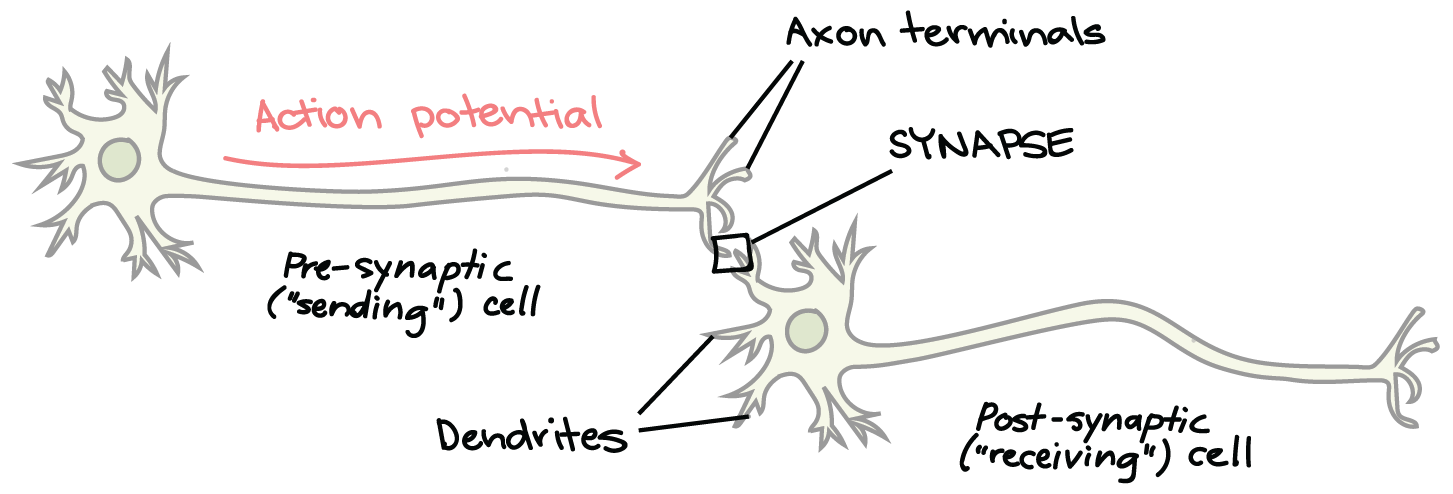
\includegraphics[width=0.7\linewidth]{img/Synapse_khan.png}
  \caption{Two neurons connected by a synapse. Image taken from Khan Academy, CC BY-NC-SA 4.0 }
  \label{fig:synapse}
\end{figure}

\noindent
In some cases this neurotransmitter will cause the post synaptic neuron to depolarise and therefore more likely to create an action potential, this is called an excitatory post synaptic potential. Otherwise the neurotransmitter will cause the membrane potential to decrease and the neuron will be less likely to create an action potential, this is called an inhibitory post synaptic potential.

\begin{figure}[ht]
  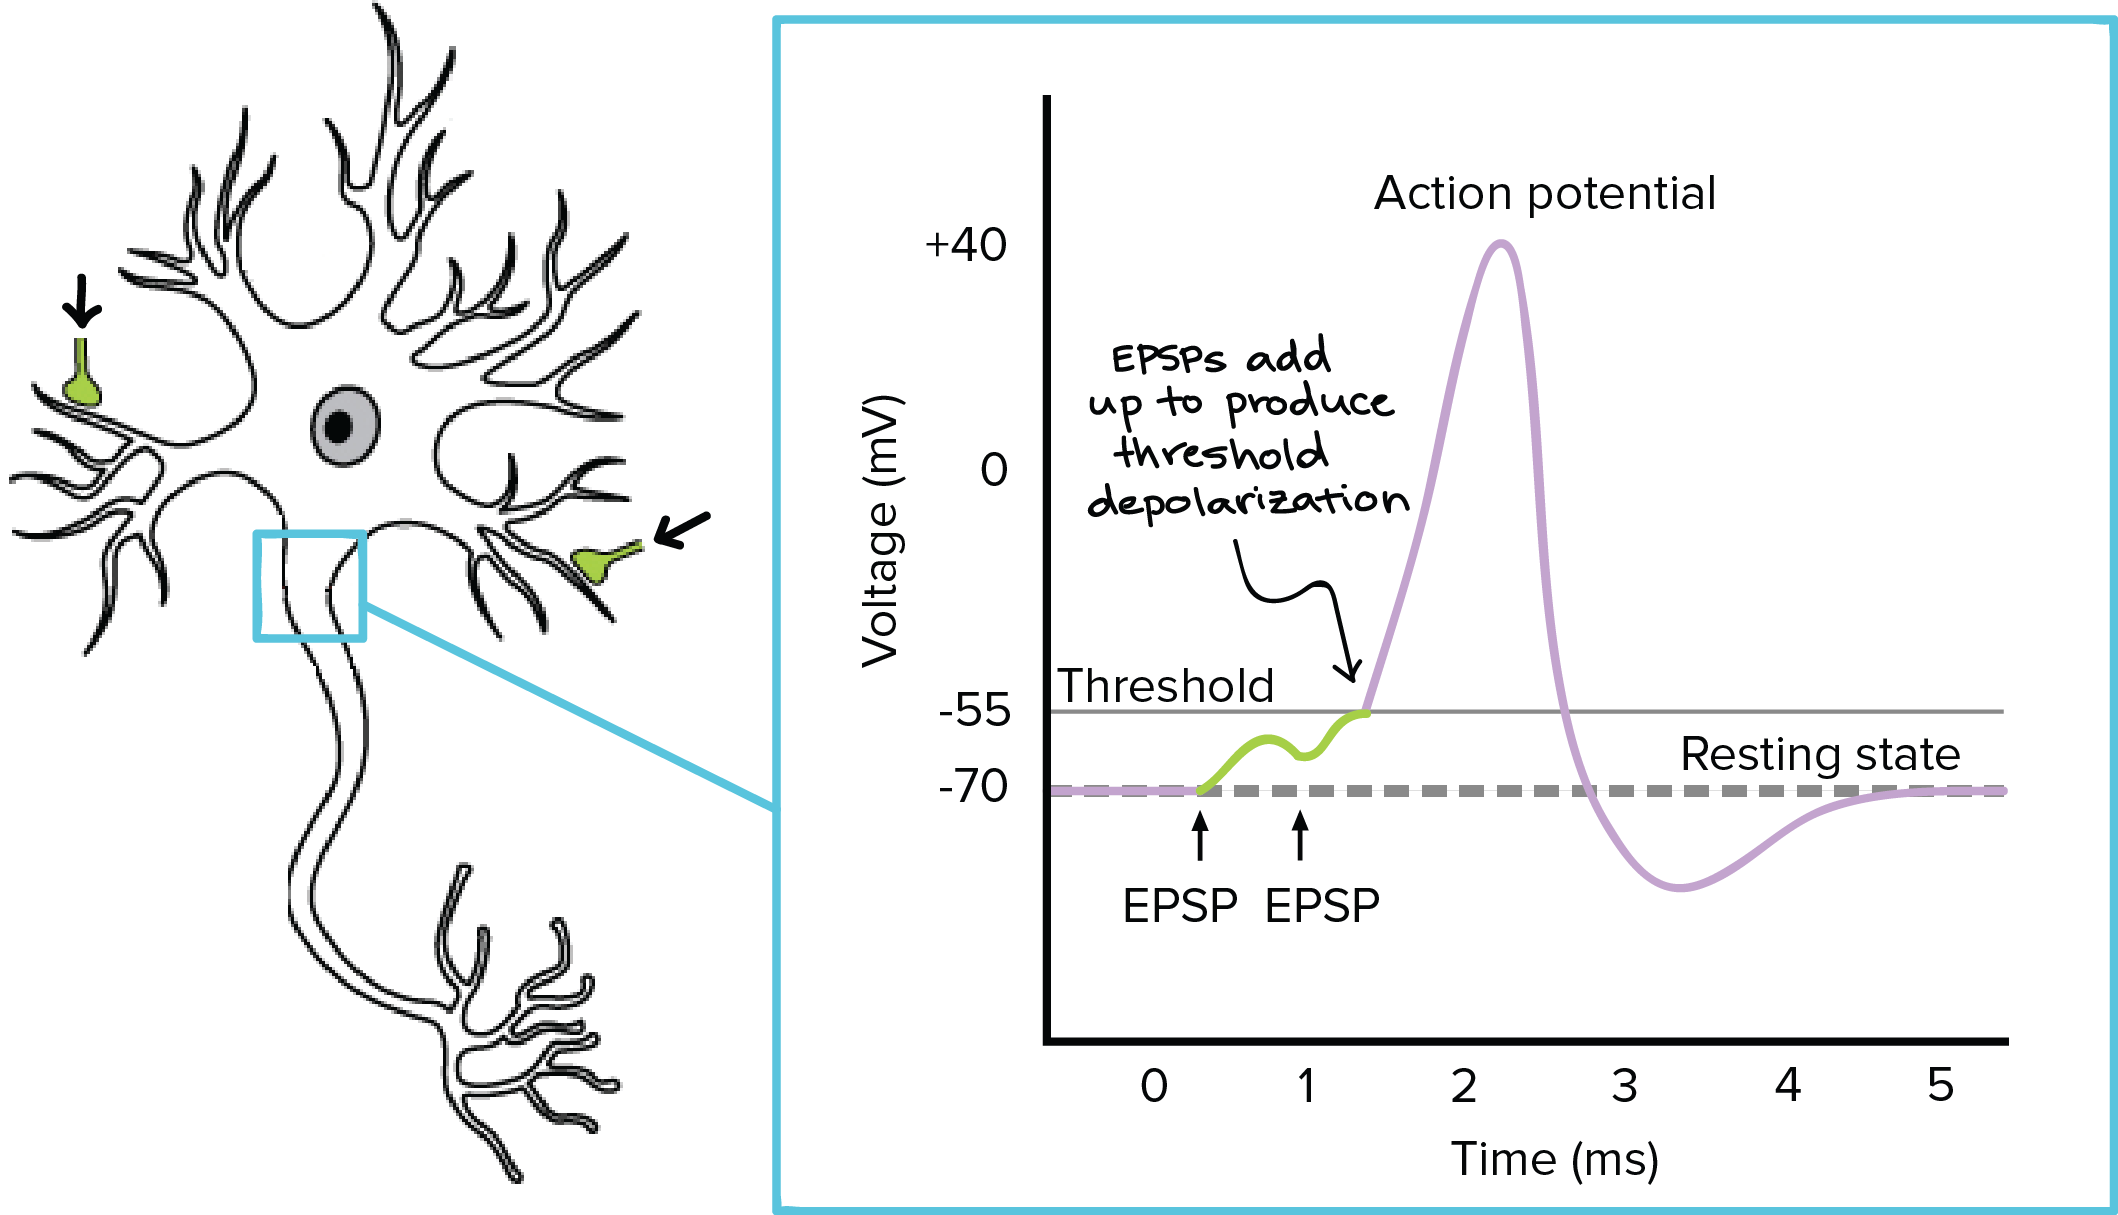
\includegraphics[width=0.7\linewidth]{img/Action_potential.png}
  \caption{A typical action potential produced from several excitatory post synaptic potentials. Image taken from Khan Academy, CC BY-NC-SA 4.0 }
  \label{fig:synapse}
\end{figure}

\section{Autism spectrum disorders}
\noindent
Autism spectrum disorders are a group of lifelong neurodevelopmental disorders. Autistic individuals often have problems with social interactions and communication, restricted interests and repetitive behaviours. The most recent prevalence studies show that 1.1\% of the UK population may be on the autism spectrum \cite{brugha2012estimating}. This is about 700,000 people and including affected families, autism spectrum disorders affect about 2.8 million people. The prevalence of autism spectrum disorders also has a marked influence on the UK economy. An individual with ASD and an intellectual disability is estimated to cost $ \pounds 1.5m $ over the course of their lifetime \cite{buescher2014costs}. These costs are mostly due to the provision of special education, lost employment (from the individual and the parents of the individual), and specialised residential care. 
\\\\
Care must be taken in steering away from the idea that autism can be cured, some see it as a normal variation in the human genome and a cure would be taking away from what makes an individual who they are. However, it cannot be ignored that ASD has a huge impact on the individuals diagnosed with the disorder, their families and society as a whole. Therefore, with more research, treatments can be developed that reduces these impacts whilst retaining the essence of the individual.
\\\\
Currently only behavioural and pharmacological treatments are available that help with the symptoms of ASD (such as anxiety and ADHD), and these are only effective for a fraction of patients. There is no known medication that can alleviate the central symptoms of autism, that is the social and communication deficits \cite{buitelaar2003have}.
\\
\section{E-I imbalance}
\noindent
Despite recent research linking several genes to autism, the underlying neurological causes are still a mystery. However, the leading theory for the aetiology of autism spectrum disorders is that there is some imbalance in the ratio of excitation to inhibition in the brain. Excitatory signals cause target neurons to fire whilst inhibitory signals suppress target neurons. The ratio of these two signals is called E-I balance. E-I balance is vital in maintaining normal brain function as it regulates the transfer of information throughout the brain. Too much excitation and neurons will constantly spike whereas if there is too much inhibition the neurons will not spike at all. In either of these states no information can be transferred (this is a similar concept to how in binary a series of just 1s or just 0s transfers no information, it is the combination of both in certain patterns that encodes data).
\\\\
An early study by Rubenstein and Merzenich \cite{rubenstein2003model} linked some forms of autism with high levels of excitation or low levels of inhibition in brain areas associated with sensory, mnemonic, social and emotional systems. They also postulated that E-I imbalance was caused by both genetic and environmental variables affecting a given neural system. Since then there has been plenty of research into the subject and any links to autism spectrum disorders.
\\\\
Excitation-inhibition imbalance has been clearly observed in mouse models of autism spectrum disorders. Pharmacological or cell type-specific gene rescue carried out on these models rescues any autistic like symptoms. These studies into animal models have shown that there is a clear link between E-I imbalance and ASD, however, they are all using invasive techniques such as optogenetics or using genetically modified mice. Obviously these techniques cannot be used in humans, and therefore, we do not know if the mechanisms studied in mice bare any relevance to ASDs in humans. Quantifying the relationship between mouse and human neurons under the influence of different E-I conditions will be the basis of this project. 
\\
\section{Integrate and fire models}
\noindent
The simplest model of a neuron is the leaky integrate and fire neuron. This was proposed in 1907 by Louis Lapicque who modelled a neuron as a resistor and capacitor in series. 
\\
\section{Project Objectives}
\noindent
The overarching aim of the research will be to investigate the links between E-I imbalance and autism spectrum disorders, and whether there is any substantial difference between the effects of E-I imbalance in human and animal models. This will be done through the use of computational models of neurons which have inputs from both excitatory and inhibitory synapses. Both mouse and human neurons will be simulated with varying inputs. The results from the models will then be compared to see if there is any difference in how sensitive the neurons are to changes in excitatory and inhibitory inputs. 
\\\\
To accomplish this a generalised leaky integrate and fire simulator will be written in Python based on the equations proposed in the Allen Institute's GLIF technical paper \cite{allen2017GLIF}. The simulator will allow for inputs from both excitatory and inhibitory synapses. The synapses will be simulated using Poisson spike trains with refractory periods. 
\\\\
The first experiment will examine the effect of changes in synaptic weight on the output of a neuron. A metric will be created for each neuron that shows how sensitive it is to changes  
\\\\
The second experiment will involve varying the firing rates of the excitatory and inhibitory synapses and observing the outputs. Again 
\\\\
Using doubly stochastic spike trains to correlate
All the experiments will be run on the 1218 neurons with GLIF models available from the Allen institute. Each experiment will be run several times and results averaged as they will be slightly different given the random nature of the Poisson inputs. Several runs of each simulation combined with the number of neurons means this will be a very compute-intensive project.

\begin{enumerate}[label=\bfseries Work package \arabic*:, align=left]
	\item Write a GLIF simulator 
	\item Stimulate the neurons using 
	
\end{enumerate}

\part{Budget}
\begin{itemize}
\item computer
\item phd student or two
\item brain simulation software. maybe 
\item cost of publishing a paper
\end{itemize}

\begin{center}
\begin{tabular}{ |p{3cm}|p{7cm}|p{3cm}|  }
 \hline
 \multicolumn{3}{|c|}{Budget} \\
 \hline
 Description & Purpose & Cost\\
 \hline
 PhD Student   & To do some research  &  $\pounds 100,000$\\
 PhD Student   & To do some research  &  $\pounds 100,000$\\
 \hline
\end{tabular}
\end{center}

\part{Justification for resources}

\part{Impact plan}
distributed to therapeutics companies?
%https://www.researchgate.net/profile/Stefano_Pallanti2/publication/283082180_Excitatoryinhibitory_imbalance_in_autism_spectrum_disorders_Implications_for_interventions_and_therapeutics/links/562dbeef08ae22b17034c69b.pdf
paper published?
\part{Work plan}
%ust pgfgantt

\bibliographystyle{angew}
\bibliography{refs}
\end{document}
